\documentclass{article}

% ── Packages ──────────────────────────────────────────────────────────────
\usepackage[utf8]{inputenc}
\usepackage[T1]{fontenc}
\usepackage{amsmath,amssymb,amsfonts}
\usepackage{graphicx}
\usepackage{booktabs}
\usepackage{multirow}
\usepackage{hyperref}
\usepackage{cleveref}
\usepackage{listings}
\usepackage{xcolor}
\usepackage{tikz}
\usepackage{float}
\usepackage{tabularx}
\usepackage{array}
\usepackage{colortbl}
\usepackage[margin=2.5cm]{geometry}
\usepackage{amsthm}

% ── Configuration listings ───────────────────────────────────────────────────
\lstset{
  basicstyle=\small\ttfamily,
  breaklines=true,
  breakatwhitespace=true,
  frame=single,
  numbers=left,
  numberstyle=\tiny\color{gray},
  captionpos=b,
  showstringspaces=false,
  language=Python,
  morekeywords={function,struct,mutable,const,for,while,if,else,elseif,end,return,using,import,export,begin,let,do},
  keywordstyle=\color{blue}\bfseries,
  comment=[l]{\#},
  commentstyle=\color{gray}\ttfamily,
  stringstyle=\color{orange},
  morestring=[b]",
  morestring=[b]',
  alsoletter={!},
  morekeywords={set!,addrule!,demand!,backward_graph!,invalidate_all!,zero_grads!,_fuse!,_watch!},
  alsoletter={_},
  morekeywords={_invalidate_downstream!,_invalidate_upstream!,patch_node!,capture_activations,recovery_metric,patch_and_measure!,restore_from_cache!,sweep_patch_sites!},
  literate={~}{{\textasciitilde}}1,
}

\definecolor{ndblue}{RGB}{30,90,180}
\definecolor{ndgreen}{RGB}{20,140,60}
\definecolor{ndred}{RGB}{190,30,30}
\definecolor{rowgray}{RGB}{245,245,245}

\newtheorem{theorem}{Theorem}
\newtheorem{corollary}{Corollary}

\title{Amortized Multi-Site Activation Patching via Cache-Replay Restoration\\in Persistent Computational Graphs}
\author{Abdallah Khemais}
\date{}

\begin{document}
\maketitle

\begin{abstract}
Activation patching localizes which internal computations of a neural network are causally
responsible for its behaviour by splicing a ``clean'' activation into a ``corrupted'' run. A
single patch is rarely the unit of interest: a causal-tracing study sweeps across every layer
(and often every position or head), running the protocol $K$ times. In tape-based frameworks
(PyTorch, JAX) and tools built on them (e.g.\ TransformerLens), each of the $K$ runs costs a full
forward pass, since the graph is rebuilt from scratch every time. \textsc{NeuroDSL}'s persistent
computational graph already makes a single patch cheap, bounding its cost by its own impact
subgraph rather than the whole network -- a direct reuse of the
$\mathcal{O}(|\mathcal{V}_{\theta}|)$ result established for parameter updates. We show that a
\emph{full sweep} carries a second, less obvious cost that this alone does not remove: restoring
the graph to its corrupted baseline between sites, if done by re-invalidating and recomputing,
pays the same order of cost as the patches themselves. Since the corrupted baseline was already
computed once and cached in full before the first patch, restoring it needs no recomputation at
all -- only a direct copy of already-known values. We introduce \texttt{restore\_from\_cache!}
and an amortized sweep orchestrator, \texttt{sweep\_patch\_sites!}, built on this observation, and
prove they leave the graph in an execution state identical to recomputation-based restoration
(exact equality, not tolerance-bounded). On an 8-layer toy Transformer, this reduces the total
cost of a full 8-site sweep by \textbf{36.1\%} (52.79~ms~$\to$~33.72~ms) on top of the
per-patch savings already available from the underlying graph, with correctness verified before
any timing claim. The same invalidation mechanism, without modification, extends to patching
several nodes at once: for two independent sites, \texttt{patch\_nodes!} composes commutatively
(exact equality regardless of application order) and its cost is bounded by the union of the
sites' cones rather than their sum, while the joint recovery it computes reflects the network's
actual nonlinear response to both interventions together, not an additive approximation. Building
on this, a greedy search over candidate sites -- \texttt{greedy\_patch\_search!} -- finds a small
combination that jointly explains most of a behaviour in a handful of steps, using an adaptive
restoration strategy that falls back to exact recomputation whenever two sites' cones overlap, a
case where the cheap cache-based restoration would otherwise silently discard an already-selected
site's active contribution. Finally, we ask whether a site's downstream cone size is itself a
signal for causal importance, independent of its already-established role as a cost proxy: across
depths, cone size closely tracks both cost and recovery, but among sibling sites at a fixed depth
-- where cone size is structurally invariant -- causal importance still varies substantially,
showing that cone size predicts recomputation cost at any depth and importance trends across
depths, but is not a substitute for direct measurement among peers. Every result above uses a
randomly-initialized network -- a valid systems benchmark, since recomputation cost depends only
on graph structure, not on weight values, but one that establishes nothing about whether the
mechanism finds anything meaningful when there is something to find. We close by training the same
architecture on the induction task, a circuit documented in the interpretability literature, and
running \texttt{greedy\_patch\_search!} unmodified over all attention heads with no positional
hint: it recovers a small set of heads reaching $99.94\%$ of the causal effect, and the two heads
found first -- confirmed by inspecting their attention patterns, a measurement entirely
independent of the search that found them -- attend with $99.8\%$ and $100\%$ weight directly to
the token position the induction algorithm must copy from. The fast mechanism this paper
introduces also finds the right answer. Since every number above comes from an 8-layer CPU model,
we additionally re-run the correctness invariants and the sweep-amortization measurement on a
$\sim$0.81-billion-parameter model on GPU: correctness holds exactly, unchanged by scale or
device, but the amortization gain drops to $9.9$--$14.3\%$ -- real, but far more modest than the
CPU figure, because a cache-replay copy that is nearly free relative to CPU recomputation is
instead a non-negligible kernel launch on GPU. We report this honestly rather than presenting the
CPU number as if it were scale-invariant.
\end{abstract}

%══════════════════════════════════════════════════════════════════════════
\section{Introduction}
\label{sec:intro}
%══════════════════════════════════════════════════════════════════════════

Mechanistic interpretability seeks to explain a neural network's behaviour by identifying which
internal computations are causally responsible for it. \textbf{Activation patching} (also called
causal tracing) \cite{rome,causalmediation} is the workhorse technique for this: run the model
once on a ``clean'' input and once on a ``corrupted'' input, then copy a single internal
activation from the clean run into the corrupted run and observe how much of the output moves
back towards the clean behaviour. The unit of a real study is not one patch but a \textbf{sweep}:
repeating this at every layer (and often every attention head or token position) to localize
where the causally relevant computation lives. Tooling such as TransformerLens
\cite{transformerlens} has made this sweep protocol a standard part of the
mechanistic-interpretability toolkit.

In tape-based frameworks, the cost of a sweep is $K$ full forward passes: PyTorch \cite{pytorch}
and JAX \cite{jax} rebuild the computational graph from nothing on every call, so patching one
node and observing the output costs exactly the same as patching any other, regardless of how
much computation actually lies downstream of the patched site.

\textsc{NeuroDSL} \cite{neurodsl} maintains a persistent, mutable computational graph in which
every node tracks whether its cached value is still valid. Writing a node invalidates only its
true downstream dependents (its impact subgraph), and the next demand-driven evaluation
recomputes exactly that subgraph -- a mechanism proven to cost
$\mathcal{O}(|\mathcal{V}_{\theta}|)$, independent of total graph size, for parameter updates
during training \cite{neurodsl}. Activation patching is, mechanically, the same operation (a node
write followed by a demand), so a single patch inherits the same bound for free.

A full sweep, however, is not just $K$ independent cheap patches: each site must be tested from a
common corrupted baseline, so the graph must be restored between sites. If restoration is done
the same way a patch is applied -- write the corrupted value back, then let the graph
re-invalidate and recompute -- it pays exactly the same recomputation cost as the patch it is
undoing. Summed across a sweep, this restoration cost is of the same order as the sweep's own
measurement cost, eating a substantial fraction of the saving a single cheap patch promised. We
show that this is avoidable: the corrupted baseline was already computed once, in full, before
the first patch. Restoring to it is not new information -- it requires no computation, only a
direct copy of values already sitting in a cache.

We make eight contributions:
\begin{enumerate}
    \item \texttt{patch\_node!} (\S\ref{sec:mechanism}), a value-injection primitive built on
    \textsc{NeuroDSL}'s existing invalidation traversal, together with the precise reason the
    graph's generic value-update primitive (\texttt{set!}) is unsuitable for this purpose.
    \item \texttt{restore\_from\_cache!} and \texttt{sweep\_patch\_sites!}
    (\S\ref{sec:sweep}), which restore a patched site's downstream cone by direct cache replay
    instead of recomputation, and an amortized sweep orchestrator built on top of it -- a
    capability specific to a persistent graph, where every node is individually addressable and
    its validity state explicit; a framework that rebuilds its graph from scratch has no
    equivalent notion of ``this node, restored, without recomputing it.''
    \item \texttt{patch\_nodes!} and \texttt{restore\_nodes\_from\_cache!} (\S\ref{sec:composable}),
    extending the same mechanism to simultaneous multi-site patches: commutative for independent
    sites, with cost bounded by the union of their cones rather than the sum, using no new
    graph-level primitive.
    \item \texttt{greedy\_patch\_search!} and \texttt{\_adaptive\_restore!} (\S\ref{sec:search}), a
    greedy search over candidate sites that restores cheaply by cache when provably safe to do so
    and falls back to exact recomputation whenever a candidate's cone overlaps an
    already-selected site's -- a case where cache-based restoration would otherwise silently
    discard the selected site's still-active contribution.
    \item A structural-signal analysis (\S\ref{sec:results}) asking whether a site's downstream
    cone size -- computable from \texttt{\_downstream\_nodes} without ever running a patched
    forward pass -- predicts its causal importance: it does across depths, closely tracking both
    cost and recovery, but among sibling sites that share a depth, where cone size is structurally
    invariant, it carries no information at all, and causal importance still requires direct
    measurement.
    \item A validation of \texttt{greedy\_patch\_search!} against a documented ground-truth
    circuit (\S\ref{sec:induction}): trained on the induction task \cite{induction}, the same
    search that operates blindly over cost and recovery recovers a small set of attention heads
    reaching $99.94\%$ of the causal effect, and the two heads it finds first are independently
    confirmed, by inspecting attention patterns the search never examined, to attend almost
    entirely to the exact token position the induction algorithm must copy from.
    \item A correctness-first empirical evaluation (\S\ref{sec:correctness}--\S\ref{sec:results})
    on a small Transformer: per-patch cost and recovery as a function of layer depth (cross-checked
    by a marginal-cost decomposition that sums to exactly the independently-measured full-forward
    cost), a 36.1\% reduction in total sweep cost from cache-replay restoration, a joint-vs-additive
    recovery comparison for two composed sites, and a 4-step greedy search trajectory whose final
    recovery is independently reproducible, with every speed number preceded by an
    exact-equality correctness check.
    \item A scale check the CPU benchmark alone cannot provide (\S\ref{sec:gpuscale}): on a
    $\sim$0.81-billion-parameter model on GPU, all correctness invariants hold exactly, unchanged
    by scale or device, but the amortization gain drops to $9.9$--$14.3\%$, far below the CPU
    figure -- traced to cache-replay's copy becoming a non-negligible GPU kernel launch rather than
    a near-free operation, not to any failure of the underlying mechanism.
\end{enumerate}

All experiments use \textsc{NeuroDSL}'s existing, already-tested \texttt{LlamaModel}
(\texttt{src/layers.jl}); no new model architecture was written for this paper. Code, tests, and
the executed notebook reproducing every number reported here are available at
\url{https://github.com/nevermind78/NeuroDSL}.

%══════════════════════════════════════════════════════════════════════════
\section{Background: Persistent Graphs and the Impact Subgraph}
\label{sec:background}
%══════════════════════════════════════════════════════════════════════════

We rely directly on the graph model introduced in \cite{neurodsl} and only restate what is
needed here. A \textsc{NeuroDSL} \texttt{NeuroGraph} stores named tensors (\texttt{GraphNode})
and transformation rules (\texttt{GraphRule}) that together define a persistent DAG. Writing a
new value to a node via \texttt{set!} triggers \texttt{\_invalidate\_downstream!}, a traversal
that clears the \texttt{valid} flag on the written node and on every node reachable from it
through the rule graph. A subsequent \texttt{demand!} call walks the (cached) topological order
and recomputes only the nodes it finds invalid, leaving everything else untouched.

\cite{neurodsl} proves that this traversal visits exactly the \textbf{impact subgraph}
$\mathcal{G}_\theta = (\mathcal{V}_\theta, \mathcal{E}_\theta)$ of the written node $\theta$ --
the set of nodes reachable from $\theta$ in the DAG -- giving a recomputation cost of
$\mathcal{O}(|\mathcal{V}_\theta| + |\mathcal{E}_\theta|)$, independent of the total graph size.
This bound was established and validated for \emph{parameter} updates during training. Activation
patching is, mechanically, also a node write followed by a demand -- so the same bound applies
directly to a patch, with no new theorem required.

%══════════════════════════════════════════════════════════════════════════
\section{Mechanism and API}
\label{sec:mechanism}
%══════════════════════════════════════════════════════════════════════════

\subsection{\texttt{patch\_node!}: Value Injection with Targeted Invalidation}

\texttt{set!} is designed to write leaf values -- inputs and parameters, nodes with no incoming
\texttt{GraphRule}. Calling it on such a node clears the node's own \texttt{valid} flag, which is
harmless there: \texttt{demand!} skips recomputing a node with no rule regardless of that flag,
so the written value survives. Patching targets an \emph{internal} node instead -- one that
already has a rule attached (e.g.\ a transformer block's residual-stream output). For such a
node, clearing its own \texttt{valid} flag is not harmless: the next \texttt{demand!} recomputes
it from that rule, using its real (still-corrupted) inputs, and the injected value is lost before
it can be observed.

\texttt{patch\_node!} avoids this without any new graph-level mechanism, only a different
composition of the existing ones: it mutates the node's \texttt{value}/\texttt{valid} fields
directly, so the node itself remains trusted and is never recomputed, and invalidates only its
true consumers by calling the existing \texttt{\_invalidate\_downstream!} on each of them
individually, rather than on the patched node itself.

\begin{lstlisting}[caption={\texttt{patch\_node!} (\texttt{src/patching.jl})},label={lst:patchnode}]
function patch_node!(g::NeuroGraph, sym::Symbol, cache; namespace=g.active_ns)
    nd = node(g, sym; namespace=namespace)
    nd.value = Backend.to_device(g.device, cache[sym])
    nd.valid = true
    nd.backwarded = false
    for (out_sym, rule) in g.rules[namespace]
        sym in rule.inputs || continue
        _invalidate_downstream!(g, out_sym, namespace)
    end
    return g
end
\end{lstlisting}

\subsection{Supporting API}

Two further functions complete the single-patch interface, both in \texttt{src/patching.jl} with
no changes to the core graph engine:
\begin{itemize}
    \item \texttt{capture\_activations(g, ns)} -- copies the value of every node in a namespace
    into a plain dictionary. The copy is not optional: \texttt{demand!} and
    \texttt{node(g,\ldots).value} return a live alias into the graph's own buffer, which a later
    evaluation can mutate in place.
    \item \texttt{recovery\_metric(patched, clean, corrupted)} -- the standard causal-tracing
    normalization, $1 - \|\text{patched} - \text{clean}\| \,/\, \|\text{corrupted} - \text{clean}\|$
    ($0$~=~no recovery, $1$~=~full recovery).
\end{itemize}

%══════════════════════════════════════════════════════════════════════════
\section{Amortizing a Full Sweep}
\label{sec:sweep}
%══════════════════════════════════════════════════════════════════════════

A sweep tests $K$ sites against the same corrupted baseline, so each site's test must end with
the graph restored to that baseline before the next site is tested. \texttt{patch\_and\_measure!}
does this the same way it applies a patch: call \texttt{patch\_node!} with the cached corrupted
value and let \texttt{demand!} recompute the downstream cone. This is correct, but it pays the
same recomputation cost the measurement step just paid -- restoring is exactly as expensive as
patching, for a value that was already known before either happened.

\subsection{\texttt{restore\_from\_cache!}: Restoration Without Recomputation}

The corrupted run was computed once, in full, before the first patch, and its entire state is
already sitting in \texttt{corrupted\_cache} via \texttt{capture\_activations}. Restoring a
patched site's downstream cone to that baseline is therefore not a computation to redo -- it is a
lookup already answered. \texttt{restore\_from\_cache!} writes the cached values directly into
each affected node and marks it valid, executing no rule:

\begin{lstlisting}[caption={\texttt{restore\_from\_cache!} and its cone (\texttt{src/patching.jl})},label={lst:restorecache}]
function _downstream_nodes(g::NeuroGraph, sym::Symbol, ns::Symbol)
    # same reachable set _invalidate_downstream! would visit, read-only
    ...
end

function restore_from_cache!(g::NeuroGraph, ns::Symbol, cache, nodes)
    for sym in nodes
        haskey(cache, sym) || continue
        nd = g.nodes[ns][sym]
        nd.value = copy(cache[sym])
        nd.valid = true
        nd.backwarded = false
    end
    return g
end
\end{lstlisting}

\texttt{\_downstream\_nodes} mirrors exactly the traversal \texttt{\_invalidate\_downstream!}
already performs -- same reachable set, same valid-gated semantics -- but read-only, so that the
set of nodes restored is, by construction, exactly the set a patch would have invalidated. This
is what makes the correctness argument in \S\ref{sec:correctness} an equality rather than an
approximation: both restoration paths act on the same node set, and the network's determinism
(no dropout at evaluation time) guarantees the cached values equal what recomputation would
produce.

This capability is specific to a persistent graph. A framework that rebuilds its computation from
scratch on every call has no individually addressable node to write a cached value into -- its
only operation is ``run the whole thing again.'' Restoration-by-cache is not a faster way to do
what a tape-based framework already does; it is an operation such a framework has no primitive
for at all.

\subsection{\texttt{sweep\_patch\_sites!}: An Amortized Sweep Orchestrator}

\texttt{sweep\_patch\_sites!} runs the standard patch-and-measure step for each site (identical to
\texttt{patch\_and\_measure!}) but restores via \texttt{restore\_from\_cache!} instead of a second
\texttt{patch\_node!}+\texttt{demand!} call:

\begin{lstlisting}[caption={\texttt{sweep\_patch\_sites!} (\texttt{src/patching.jl})},label={lst:sweep}]
function sweep_patch_sites!(g, output_sym, sites, clean_cache, corrupted_cache,
                             clean_output, corrupted_output; namespace=g.active_ns)
    results = NamedTuple[]
    for site in sites
        affected = _downstream_nodes(g, site, namespace)
        patch_node!(g, site, clean_cache; namespace=namespace)
        patched_output = demand!(g, output_sym; namespace=namespace)
        recovery = recovery_metric(patched_output, clean_output, corrupted_output)
        restore_from_cache!(g, namespace, corrupted_cache, affected)
        push!(results, (; site, recovery))
    end
    return results
end
\end{lstlisting}

Only the restoration step changes; the measurement step -- the actual scientific quantity of
interest -- is untouched.

%══════════════════════════════════════════════════════════════════════════
\section{Composable Multi-Site Patching}
\label{sec:composable}
%══════════════════════════════════════════════════════════════════════════

Many causal-tracing protocols beyond a single-site sweep -- path patching and its variants --
need to patch several nodes at once and observe their joint effect. The invalidation mechanism
underlying \texttt{patch\_node!} never assumed a single node changes at a time:
\texttt{\_invalidate\_downstream!} marks a node invalid regardless of how many sources triggered
it, and \texttt{demand!} visits each node in topological order exactly once, recomputing only
those still marked invalid. Patching several nodes and calling \texttt{demand!} once therefore
already computes the union of their downstream cones correctly, with any shared descendant
recomputed only once -- no new fusion logic is required for this, only an API that exposes it.

\begin{lstlisting}[caption={\texttt{patch\_nodes!} and \texttt{restore\_nodes\_from\_cache!} (\texttt{src/patching.jl})},label={lst:multipatch}]
function patch_nodes!(g::NeuroGraph, syms, cache; namespace=g.active_ns)
    for sym in syms
        patch_node!(g, sym, cache; namespace=namespace)
    end
    return g
end

function restore_nodes_from_cache!(g::NeuroGraph, ns::Symbol, cache, syms)
    affected = Set{Symbol}()
    for sym in syms
        union!(affected, _downstream_nodes(g, sym, ns))
    end
    restore_from_cache!(g, ns, cache, affected)
    return g
end
\end{lstlisting}

\paragraph{Independent sites commute; nested sites apply in list order.} For two sites where
neither is reachable from the other -- e.g.\ two attention heads of the same layer, both computed
from the same upstream projection and merged only downstream by \texttt{hcat\_heads} -- applying
\texttt{patch\_nodes!([A, B], \ldots)} and \texttt{patch\_nodes!([B, A], \ldots)} produce
identical results, since neither patch's invalidation can ever reach the other's node. For two
sites in an ancestor-descendant relationship, \texttt{patch\_nodes!} applies patches in list
order: a later entry that lies downstream of an earlier one is not affected by it, but a later
entry that lies \emph{upstream} of an earlier one will re-invalidate it, and the earlier
(downstream) patch is recomputed from the newly patched ancestor rather than kept pinned. This is
the same, well-defined semantics as any sequential in-place update -- the last write to a given
location wins -- and it is precisely why \Cref{sec:results} evaluates the commuting case, where
the interaction being measured is the sites' joint causal effect, not an artifact of application
order.

%══════════════════════════════════════════════════════════════════════════
\section{Automated Multi-Site Search}
\label{sec:search}
%══════════════════════════════════════════════════════════════════════════

A combined patch of $m$ sites costs at most the sum of their individual costs, and typically less
when their cones overlap (\Cref{sec:composable}). This makes it practical to search over
combinations of sites rather than rely solely on independent single-site attributions:
\texttt{greedy\_patch\_search!} iteratively adds, from a candidate pool, whichever remaining site
most increases the joint recovery of the sites already selected, stopping once no candidate
improves on the current best.

\paragraph{An adaptive heuristic, not a provably near-optimal one.} The cost side of this
property -- $|\text{cone}(A) \cup \text{cone}(B)| \le |\text{cone}(A)| + |\text{cone}(B)|$ -- is a
coverage function, the canonical example of a submodular set function, which is why combining
sites is never more expensive than treating them independently. It is tempting to read this as
licensing the classical greedy guarantee for submodular maximization (a $1 - 1/e$ approximation to
the optimal set \cite{submodular}): but that guarantee applies to the function being
\emph{maximized}, and here that is recovery, not cost. Nothing in this paper establishes that
recovery is submodular in the set of patched sites -- it is a property of the network's nonlinear
response (\Cref{sec:composable} already shows it is not even additive), not a counting function
over reachable nodes. \texttt{greedy\_patch\_search!} is therefore an adaptive greedy heuristic
with no proven approximation guarantee, despite superficially resembling a setting where one would
exist; its trajectory (\Cref{sec:results}) is validated empirically, by independent recomputation
(Invariant 5), not by appeal to a theorem it does not satisfy.

\paragraph{Restoring a candidate tested on top of an existing selection.} Each step of the search
tests a candidate \emph{on top of} whatever sites are already selected and still active --
different from every earlier use of \texttt{restore\_from\_cache!} in this paper, which always
restored from the fully corrupted baseline (Invariant 3, \S\ref{sec:correctness}). If the
candidate's cone overlaps a selected site's cone -- unavoidable once two sites share a downstream
merge point, as in \Cref{sec:composable} -- restoring the candidate from the corrupted cache would
also reset the shared region to its \emph{fully} corrupted value, discarding the selected site's
still-active contribution to that region. This is not a defect in \texttt{restore\_from\_cache!}:
its guarantee (Invariant 3) was always specific to undoing one patch from a fully corrupted
baseline, and it continues to hold exactly there. \texttt{\_adaptive\_restore!} applies it only
where that guarantee holds -- comparing the candidate's cone against the union of already-selected
cones (a set computation, no graph evaluation) -- and falls back to recomputation-based
restoration, which remains correct regardless of overlap, everywhere else.

\begin{lstlisting}[caption={\texttt{\_adaptive\_restore!} and \texttt{greedy\_patch\_search!} (\texttt{src/patching.jl})},label={lst:greedy}]
function _adaptive_restore!(g, ns, cand, cand_cone, selected_cone_union, corrupted_cache, output_sym)
    if isempty(intersect(cand_cone, selected_cone_union))
        restore_from_cache!(g, ns, corrupted_cache, cand_cone)
    else
        patch_node!(g, cand, corrupted_cache; namespace=ns)
        demand!(g, output_sym; namespace=ns)
    end
    return g
end

function greedy_patch_search!(g, output_sym, candidates, clean_cache, corrupted_cache,
                               clean_output, corrupted_output; max_sites=length(candidates),
                               namespace=g.active_ns)
    selected = Symbol[]; remaining = collect(candidates)
    trajectory = NamedTuple[]; best_so_far = 0.0
    selected_cone_union = Set{Symbol}()
    for _ in 1:max_sites
        best_site = nothing; best_recovery = best_so_far
        for cand in remaining
            cand_cone = _downstream_nodes(g, cand, namespace)
            patch_node!(g, cand, clean_cache; namespace=namespace)
            r = recovery_metric(demand!(g, output_sym; namespace=namespace),
                                 clean_output, corrupted_output)
            _adaptive_restore!(g, namespace, cand, cand_cone, selected_cone_union,
                                corrupted_cache, output_sym)
            r > best_recovery && ((best_recovery, best_site) = (r, cand))
        end
        best_site === nothing && break
        best_cone = _downstream_nodes(g, best_site, namespace)
        patch_node!(g, best_site, clean_cache; namespace=namespace)
        demand!(g, output_sym; namespace=namespace)
        push!(selected, best_site); filter!(s -> s != best_site, remaining)
        union!(selected_cone_union, best_cone); best_so_far = best_recovery
        push!(trajectory, (; site=best_site, cumulative_recovery=best_recovery))
    end
    return selected, trajectory
end
\end{lstlisting}

%══════════════════════════════════════════════════════════════════════════
\section{Correctness Validation}
\label{sec:correctness}
%══════════════════════════════════════════════════════════════════════════

Following the same discipline as \cite{neurodsl} -- correctness before any speed claim -- every
mechanism in this paper is validated by an invariant that does not depend on comparing two
implementations that could share the same flaw.

\paragraph{Invariant 1: the patched value survives evaluation.} After
\texttt{patch\_node!(g, sym, clean\_cache)}, we compare \texttt{node(g, sym).value} immediately
after the patch to the same value \emph{after} a subsequent \texttt{demand!(g, output)} call.
These must be identical -- if \texttt{demand!} recomputed the node, they would differ. Measured
maximum absolute difference: $\mathbf{0.0}$ (exact).

\paragraph{Invariant 2: patching the last layer is patching the output.} In our test model, the
output node \emph{is} the last transformer block's residual-stream output
(\texttt{layer\_\{n\}\_out}); patching one is, structurally, patching the other. Recovery must
equal exactly $1.0$ -- a mathematical identity, not a second implementation. Measured:
$\mathbf{1.000000}$.

\paragraph{Invariant 3: cache-replay restoration equals recomputation-based restoration.} For the
same site, patched from the same corrupted baseline, we compare the full graph state (every
node's value) after restoring via \texttt{restore\_from\_cache!} against the state after
restoring via \texttt{patch\_node!}+\texttt{demand!}. Every node matches exactly. This is the
invariant that licenses the sweep result of \S\ref{sec:results}: the two restoration paths are
interchangeable in outcome, so any wall-clock difference between them is pure overhead removed,
not a shortcut that changes what is being measured.

\paragraph{Invariant 4: independent patches compose commutatively.} For two sibling attention
heads of the same layer (\S\ref{sec:composable}), we compare the output after
\texttt{patch\_nodes!([A, B], \ldots)} against the output after applying the same two patches in
reverse list order. The two match exactly, confirming that neither patch's invalidation reaches
the other's node.

\paragraph{Invariant 5: the search's reported recovery is independently reproducible.} After
\texttt{greedy\_patch\_search!} returns its selected sites, we patch all of them at once via
\texttt{patch\_nodes!} on a graph freshly reset to the corrupted baseline -- a code path entirely
separate from the search's internal bookkeeping -- and recompute recovery. This matches the
search's own final trajectory value exactly, confirming that the adaptive restoration used
internally never left the graph in a state that would misreport the outcome.

All five invariants were confirmed before any timing measurement was taken.

%══════════════════════════════════════════════════════════════════════════
\section{Experimental Setup}
\label{sec:setup}
%══════════════════════════════════════════════════════════════════════════

We use \textsc{NeuroDSL}'s existing, already-tested \texttt{LlamaModel} (8 layers, hidden
dimension 128, 8 attention heads, sequence length 16; \texttt{src/layers.jl}) -- no new
architecture was written for this paper. The model is fed a random $(16, 128)$ matrix directly
as its input node, with no token or positional embeddings and no output head, since demonstrating
the systems capability requires no language-modelling semantics.

\paragraph{Corruption protocol.} We generate a clean input, then corrupt it by replacing a single
token's row (position~1) with fresh noise -- the standard single-token causal-tracing protocol.

\paragraph{Patch granularity.} Cost is measured by patching each layer's entire output tensor
(all token positions at once), since cost does not depend on which positions are patched, only on
how much computation lies downstream. Recovery is measured by patching only the corrupted
token's row, leaving all other positions as the corrupted run computed them: replacing a layer's
entire output with its clean counterpart makes every subsequent computation identical to the
clean run by determinism, which is the correct behaviour but gives no depth-dependent signal --
patching only the affected position is what reveals where its influence is reintegrated into the
network.

%══════════════════════════════════════════════════════════════════════════
\section{Results}
\label{sec:results}
%══════════════════════════════════════════════════════════════════════════

\subsection{Single-Site Cost and Recovery vs.\ Depth}

\Cref{tab:results} reports, for each layer, the size of its downstream cone
$|\mathcal{V}_\theta|$ (\texttt{\_downstream\_nodes}, computed read-only before patching), the
wall-clock cost of patching that layer's output and recomputing the model's output (trimmed mean
over 15 alternated runs, following the warm-up and alternation discipline of \cite{neurodsl} to
control for CPU clock variance), and the recovery achieved by patching only the corrupted token's
position. The reference full-forward cost -- the cost of a complete forward pass, i.e.\ what every
site in this table would cost under full re-invalidation -- is measured with the same rigor as
every other timing in this paper (dedicated warm-up, alternating clean/corrupted runs, trimmed
mean over 15 runs): $6.201 \pm 0.302$~ms for this run.

\begin{table}[H]
\centering
\caption{Patch cost, downstream cone size, and recovery vs.\ layer depth, 8-layer
\texttt{LlamaModel} (dim=128).}
\label{tab:results}
\begin{tabular}{c c c c c}
\toprule
\textbf{Layer} & \textbf{Cone size} & \textbf{Cost (ms)} & \textbf{Cost (\% of full forward)} & \textbf{Recovery} \\
\midrule
1 & 484 & 5.418 & 87.4\% & 0.753 \\
2 & 415 & 4.606 & 74.3\% & 0.666 \\
3 & 346 & 3.831 & 61.8\% & 0.613 \\
\rowcolor{rowgray}
4 & 277 & 3.071 & 49.5\% & 0.565 \\
5 & 208 & 2.191 & 35.3\% & 0.521 \\
6 & 139 & 1.444 & 23.3\% & 0.461 \\
7 & 70  & 0.734 & 11.8\% & 0.435 \\
8 & 1   & 0.000 & 0.0\%  & 0.386 \\
\bottomrule
\end{tabular}
\end{table}

\begin{figure}[H]
\centering

\includegraphics[width=0.49\textwidth]{figures/patching_cost.pdf}
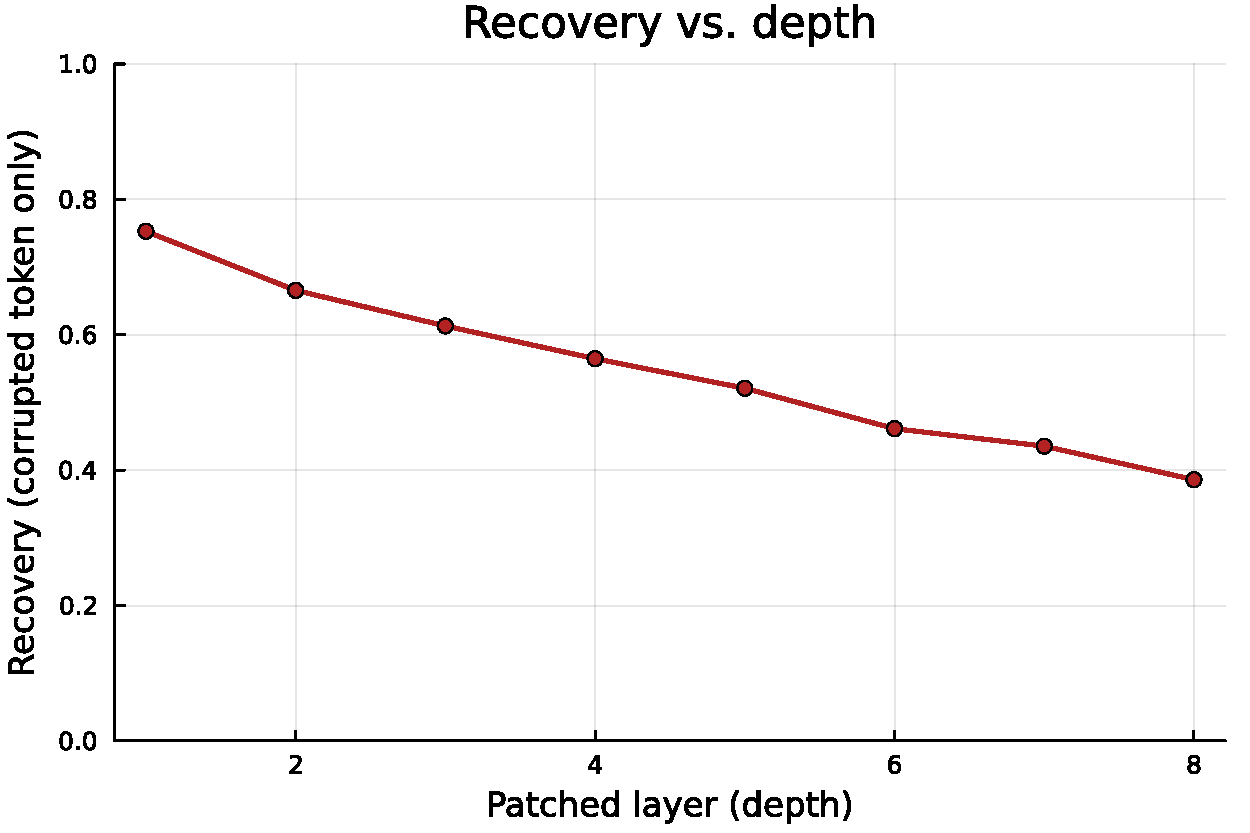
\includegraphics[width=0.49\textwidth]{figures/patching_recovery.pdf}
\caption{Left: patch cost as a percentage of a full forward pass, by layer depth. Right:
recovery of the corrupted token's position, by layer depth. Both decrease monotonically with
depth; cost reaches exactly zero at the output layer, where nothing remains downstream to
recompute.}
\label{fig:results}
\end{figure}

Cost decreases monotonically with depth, reaching exactly $0.0\%$ at the output layer, where the
impact subgraph is empty by definition. Recovery of the single corrupted token also decreases
with depth, consistent with restoring the corrupted position earlier giving the network's own
unmodified computation more opportunity to reintegrate the correction.

\paragraph{Marginal cost: a cross-check on measurement rigor.} The cost column of
\Cref{tab:results} is cumulative: patching layer $i$ recomputes the entire downstream suffix
$i{+}1, \ldots, 8$, so consecutive rows overlap and the column has no reason to sum to any
particular total. The \emph{marginal} cost of layer $i$ -- the computation specific to that layer
alone, disjoint from every other layer -- is instead the difference between consecutive cumulative
costs, $\text{marginal}(i) = \text{cumulative}(i{-}1) - \text{cumulative}(i)$, with
$\text{cumulative}(0)$ taken to be the full-forward cost and $\text{cumulative}(8) = 0$ (patching
the last layer is patching the output). Marginal and cumulative cost are a discrete derivative and
its corresponding sum: $\text{marginal}$ is the backward difference of $\text{cumulative}$, so by
the discrete analogue of the fundamental theorem of calculus, summing it back up telescopes to
$\text{cumulative}(0) - \text{cumulative}(8)$ regardless of the particular values in between --
i.e.\ exactly the full-forward cost, for any monotone nested cost sequence, not a property special
to this measurement. \Cref{tab:marginal} reports this decomposition; comparing its sum against the
full-forward cost measured independently above ($6.201$~ms) serves as a cross-check on measurement
consistency, over and above the per-invariant correctness checks of \S\ref{sec:correctness}.

\begin{table}[H]
\centering
\caption{Marginal cost per layer -- disjoint contributions that sum to the full-forward cost.}
\label{tab:marginal}
\begin{tabular}{c c c}
\toprule
\textbf{Layer} & \textbf{Marginal cost (ms)} & \textbf{Marginal cost (\% of full forward)} \\
\midrule
1 & 0.783 & 12.6\% \\
2 & 0.812 & 13.1\% \\
\rowcolor{rowgray}
3 & 0.775 & 12.5\% \\
4 & 0.760 & 12.3\% \\
5 & 0.880 & 14.2\% \\
\rowcolor{rowgray}
6 & 0.746 & 12.0\% \\
7 & 0.710 & 11.4\% \\
8 & 0.734 & 11.8\% \\
\midrule
\textbf{Sum} & \textbf{6.200} & \textbf{100.0\%} \\
\bottomrule
\end{tabular}
\end{table}

The sum matches the independently-measured full-forward cost ($6.201$~ms) to within $0.001$~ms --
consistent with the two quantities being the same underlying cost decomposed two different ways,
not two unrelated numbers that happen to agree.

\subsection{Amortized Sweep Cost}

\Cref{tab:sweep} compares the total wall-clock cost of a full 8-site sweep (patching every
layer's output once, in sequence) under the two restoration strategies of \S\ref{sec:sweep},
trimmed mean over 10 alternated runs.

\begin{table}[H]
\centering
\caption{Total cost of an 8-site sweep, by restoration strategy.}
\label{tab:sweep}
\begin{tabular}{l c}
\toprule
\textbf{Restoration strategy} & \textbf{Total sweep cost (ms)} \\
\midrule
Recomputation (\texttt{patch\_node!} + \texttt{demand!}) & 52.79 $\pm$ 1.49 \\
\rowcolor{rowgray}
Cache replay (\texttt{restore\_from\_cache!}) & \textbf{33.72 $\pm$ 2.24} \\
\bottomrule
\end{tabular}
\end{table}

\begin{figure}[H]
\centering
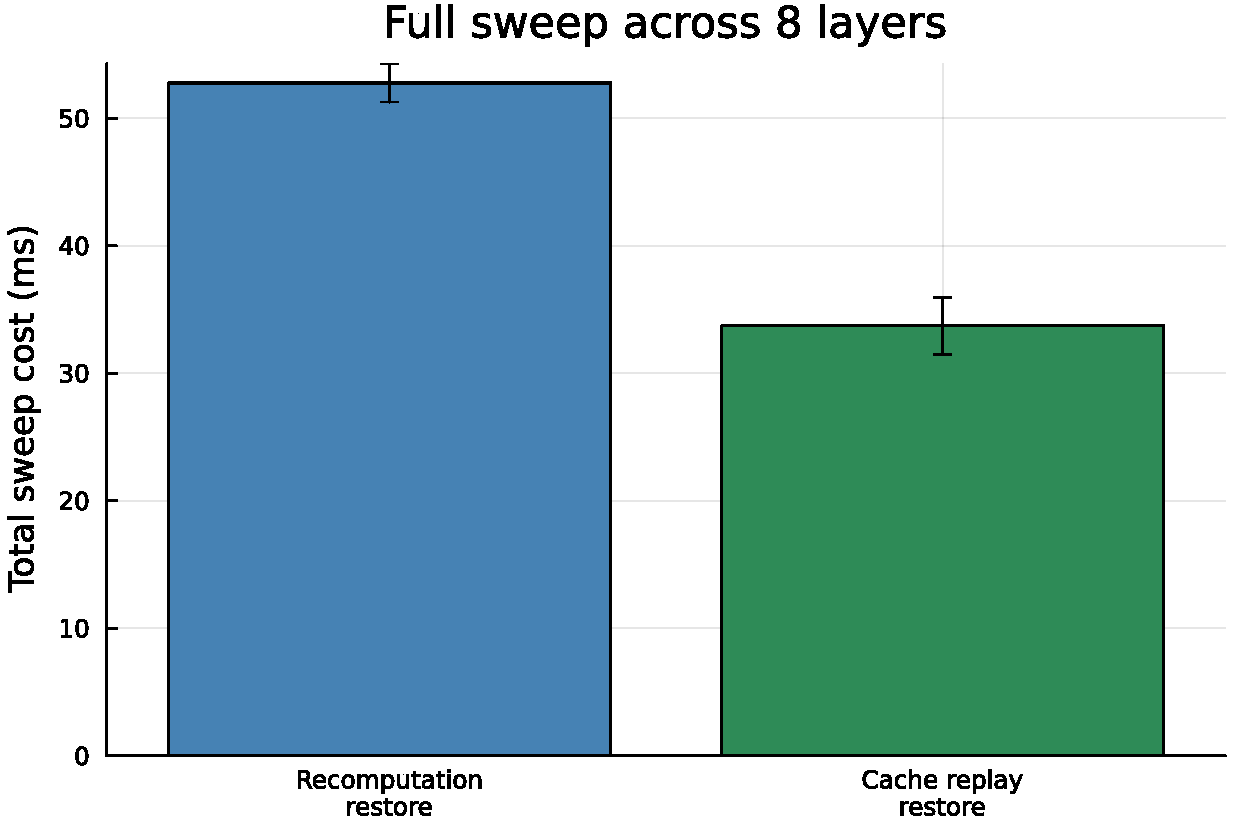
\includegraphics[width=0.6\textwidth]{figures/patching_sweep_cost.pdf}
\caption{Total cost of a full 8-site sweep, recomputation-based restoration vs.\ cache-replay
restoration.}
\label{fig:sweep}
\end{figure}

Cache-replay restoration reduces total sweep cost by \textbf{36.1\%} relative to
recomputation-based restoration, verified (Invariant 3, \S\ref{sec:correctness}) to leave the
graph in an identical state either way. This gain is additive to the per-patch savings already
demonstrated in \Cref{tab:results}: the measurement side of the sweep is untouched, only the
restoration side's redundant recomputation is removed.

\subsection{Composable Multi-Site Patching}

We patch two sibling attention heads of the same layer (\texttt{layer\_1\_mha\_ao\_h2} and
\texttt{layer\_1\_mha\_ao\_h3}, \S\ref{sec:composable}), individually and jointly, each with only
the corrupted token's position restored to its clean value.

\begin{table}[H]
\centering
\caption{Individual vs.\ joint recovery for two sibling attention heads.}
\label{tab:composable}
\begin{tabular}{l c}
\toprule
\textbf{Patch} & \textbf{Recovery} \\
\midrule
Head 2 alone & 0.0295 \\
Head 3 alone & 0.0427 \\
Additive sum (head 2 + head 3) & 0.0723 \\
\rowcolor{rowgray}
Both heads, jointly (\texttt{patch\_nodes!}) & \textbf{0.0647} \\
\bottomrule
\end{tabular}
\end{table}

The joint patch's recovery ($0.0647$) is below the additive sum of the two individual recoveries
($0.0723$), confirming that \texttt{patch\_nodes!} computes the network's actual joint response
to both interventions together, rather than a superposition of two independently-measured
effects -- a distinction that only matters because the underlying computation (attention,
normalization, the residual stream) is nonlinear.

The two heads' downstream cones overlap almost entirely (both merge at the same
\texttt{hcat\_heads} node): $493$ nodes each, for a combined size of $986$ if handled
independently, against a union of $494$ -- patching both at once, restoring their shared cone
once, costs essentially half of treating them as two unrelated single-site patches.

\subsection{Automated Multi-Site Search}

\Cref{tab:greedy} reports the trajectory of \texttt{greedy\_patch\_search!} over the 8 attention
heads of a single layer: at each step, the head added is whichever most increases cumulative
recovery, and the search stops once none of the remaining heads improve on the current best.

\begin{table}[H]
\centering
\caption{Greedy search trajectory over 8 candidate attention heads (one layer).}
\label{tab:greedy}
\begin{tabular}{c l c}
\toprule
\textbf{Step} & \textbf{Site added} & \textbf{Cumulative recovery} \\
\midrule
1 & Head 3 & 0.0427 \\
\rowcolor{rowgray}
2 & Head 5 & 0.0682 \\
3 & Head 2 & 0.0864 \\
\rowcolor{rowgray}
4 & Head 8 & 0.0977 \\
\bottomrule
\end{tabular}
\end{table}

The search stops after 4 of the 8 candidate heads: none of the remaining 4 improve on a
cumulative recovery of $0.0977$. Recomputing this same combination independently via
\texttt{patch\_nodes!}, on a graph freshly reset to the corrupted baseline, gives an identical
$0.0977$ (Invariant 5, \S\ref{sec:correctness}) -- the adaptive restoration used during the
search, including the cases where it fell back to recomputation because two heads' cones
overlapped, never desynchronized the graph from what an independent recomputation would report.

\subsection{Structural Signal: Cone Size vs.\ Causal Importance}

Every result so far concerns the cost of computation, not what that cost implies about a site's
causal importance. Since \Cref{tab:results} already reports each layer's downstream cone size
$|\mathcal{V}_\theta|$ alongside its cost and recovery, a natural question is whether cone size
itself -- computable from \texttt{\_downstream\_nodes} without ever running a patched forward
pass -- is a signal for causal importance, or only for recomputation cost.

Across the 8 layers, cone size correlates almost perfectly with cost ($r=0.9997$, as expected:
both count the same recomputed node set, one by an integer tally and the other by wall-clock
time) and closely with recovery ($r=0.9928$). This second correlation is confounded, though: cost
and recovery both decrease with depth in \Cref{tab:results}, so any two quantities that track
depth will appear correlated with each other. A more informative test holds depth fixed and asks
whether cone size still discriminates importance among sites that share it.

\Cref{tab:heads} repeats the corrupted-token-only recovery protocol of \S\ref{sec:setup} on each
of the 8 attention heads of layer 1 individually (rather than in combination, as in
\S\ref{sec:composable}--\S\ref{sec:search}). Because all 8 heads merge into the same downstream
chain (\texttt{hcat\_heads}, then layers 2--8), their downstream cones are not merely similar but
\emph{identical} in size -- $493$ nodes for every head, confirmed directly. Their individual
recoveries, in contrast, vary meaningfully -- and even in sign, ranging from $-0.0082$ to
$+0.0237$ -- reflecting the small, sometimes destructive contribution a single head makes to a
single token position in a randomly-initialized network.

\begin{table}[H]
\centering
\caption{Downstream cone size and individual recovery for 8 sibling attention heads (layer 1,
depth held fixed).}
\label{tab:heads}
\begin{tabular}{c c c}
\toprule
\textbf{Head} & \textbf{Cone size} & \textbf{Recovery} \\
\midrule
1 & 493 & $-0.0071$ \\
2 & 493 & $+0.0200$ \\
\rowcolor{rowgray}
3 & 493 & $+0.0237$ \\
4 & 493 & $-0.0082$ \\
5 & 493 & $+0.0198$ \\
\rowcolor{rowgray}
6 & 493 & $-0.0029$ \\
7 & 493 & $+0.0019$ \\
8 & 493 & $+0.0108$ \\
\bottomrule
\end{tabular}
\end{table}

\begin{figure}[H]
\centering
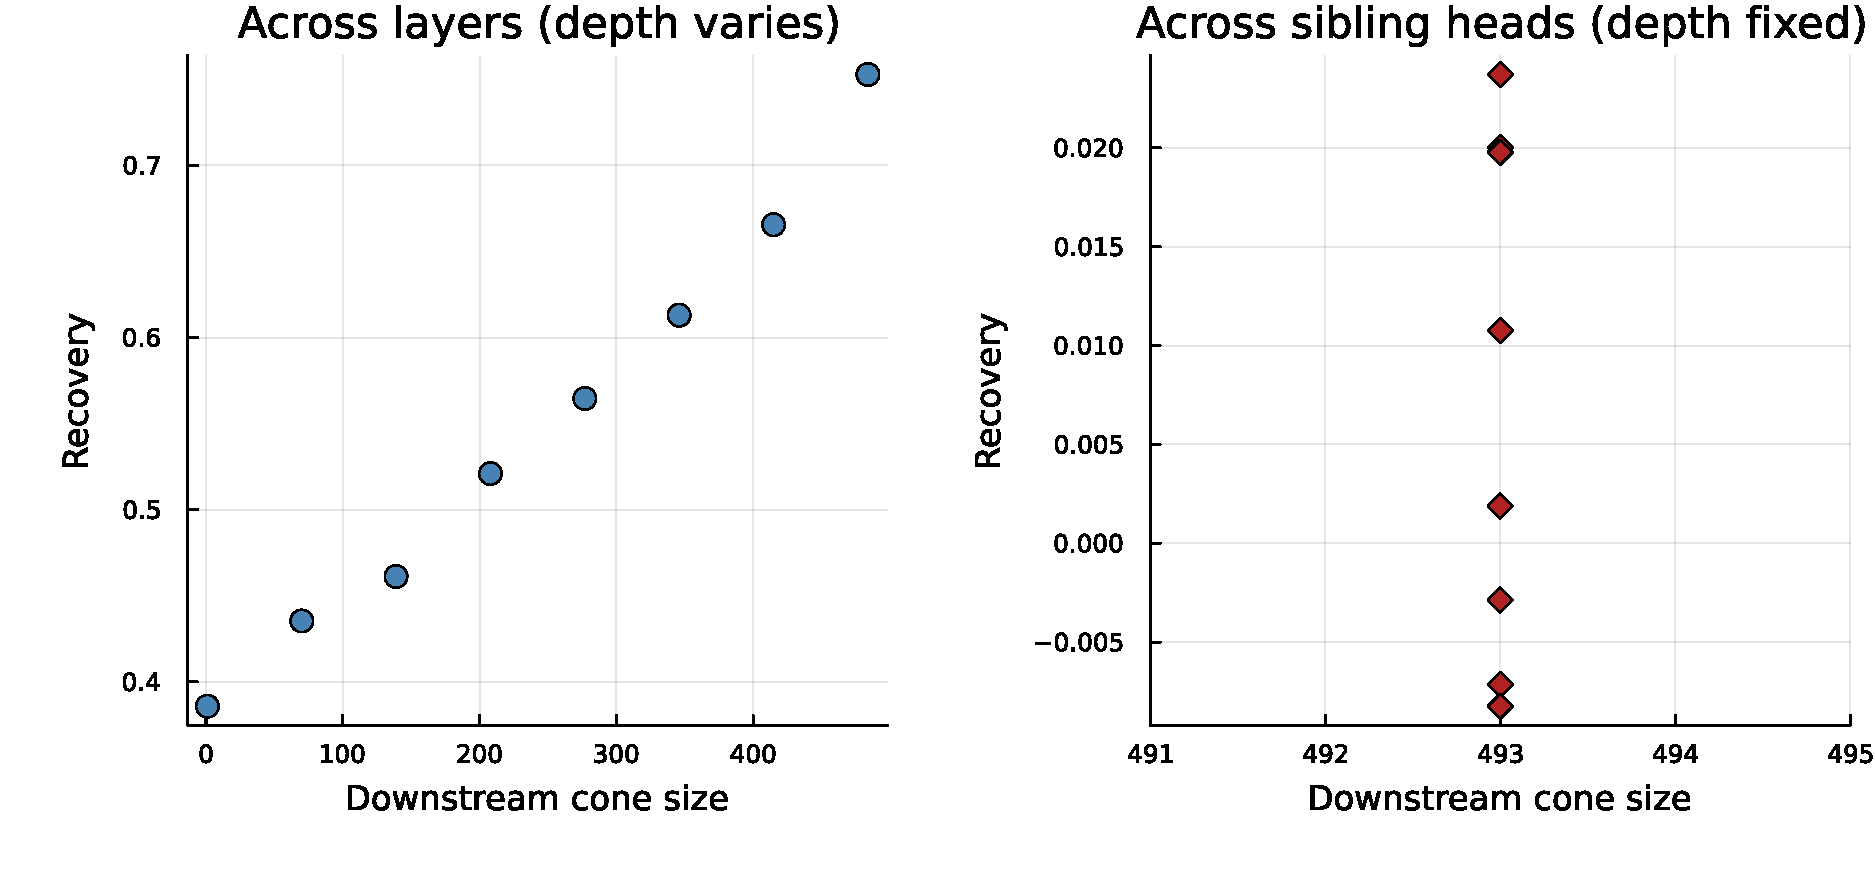
\includegraphics[width=0.9\textwidth]{figures/patching_structural_signal.pdf}
\caption{Downstream cone size vs.\ recovery. Left: across the 8 layers of \Cref{tab:results},
where depth drives both quantities together. Right: across the 8 sibling heads of
\Cref{tab:heads}, where cone size is constant but recovery still varies.}
\label{fig:structural}
\end{figure}

\Cref{fig:structural} makes the contrast visible: a clear downward trend across layers (left),
collapsing to a single vertical line of points across sibling heads (right), where cone size
carries no information at all. Cone size is therefore a reliable, hardware-independent proxy for
recomputation cost at any depth, and it tracks the trend of causal importance across depths -- but
among sites that share a depth, distinguishing which one matters still requires the direct
measurement this paper's mechanism makes cheap, not a structural shortcut around it.

%══════════════════════════════════════════════════════════════════════════
\section{Validating Circuit Discovery on a Known Task}
\label{sec:induction}
%══════════════════════════════════════════════════════════════════════════

Everything so far demonstrates that the patching mechanism is fast and correct on a
randomly-initialized \texttt{LlamaModel} -- a valid systems benchmark, since recomputation cost
depends only on graph structure, not on weight values, but one that establishes nothing about
whether the mechanism finds anything meaningful when there is something to find. We now train the
same architecture on a task with a documented ground-truth circuit and ask whether
\texttt{greedy\_patch\_search!}, unmodified, recovers it.

\subsection{Task and Training}

Induction task \cite{induction}: sequence = random prefix of length $P$ over a small vocabulary,
repeated once (total length $2P$); predicting the next token on the second half is solvable only
by induction (find the previous occurrence of the current token, copy what followed it) -- causal
attention guarantees the first half is unpredictable by construction, since no earlier occurrence
exists to copy from. We add an \texttt{Embedding} layer (new, \texttt{src/layers.jl}, wired on
\textsc{NeuroDSL}'s existing \texttt{:embedding} op, previously present only as a low-level
primitive with no high-level struct) for tokens and positions, keep \texttt{LlamaModel} unchanged
(3 layers, hidden dimension 64, 4 heads, vocabulary 20, prefix length 8), and train with the AdamW
step primitives already present in the codebase (\texttt{backward\_graph!},
\texttt{adamw\_step!}), resampling a fresh random prefix every step so the model must learn the
general algorithm rather than memorize token statistics.

\subsection{Confirming Genuine Generalization}

On 100 freshly sampled sequences, never seen during training: $100.0\%$ next-token accuracy on
the second half (the repeat), versus $16.4\%$ on the first half (chance is $5\%$ at vocabulary
size 20; the small excess reflects incidental within-prefix repeats). This asymmetry -- solved
where solvable, near-chance where not -- is the signature of a learned in-context algorithm, not
memorization of a fixed training set. We verify this before any causal analysis, the same
discipline applied to correctness throughout this paper.

\subsection{Locating the Circuit}

We construct a clean/corrupted pair by the same single-token protocol as \S\ref{sec:setup}: a
fresh test sequence, corrupted by replacing the token at the position the induction mechanism must
copy from ($i_{\text{src}}$), and probe the model's prediction at the corresponding target
position $j$ (the first position of the repeated half). The corruption flips the model's top
prediction at $j$, giving a clean recovery target.

Two adaptations follow from a real algorithm being present rather than noise. First,
\texttt{recovery\_metric} is applied to row $j$ of the logits rather than the whole output: causal
attention propagates the corruption to every position after $i_{\text{src}}$, so comparing full
output tensors would mix the induction-specific effect with generic downstream drift; slicing to
the one prediction of interest isolates it, reusing \texttt{recovery\_metric} unchanged, only on a
narrower view. Second, patching a layer's residual stream at the \emph{source} position
$i_{\text{src}}$ recovers essentially nothing ($\le 0.001$ at every layer), while patching the same
layer at the \emph{target} position $j$ recovers $98.5\%$ already at layer 1 (\Cref{tab:induction-layers})
-- the corrected information only becomes causally load-bearing once attention has moved it to the
position that reads it; patching where it originated, before that read happens, patches nothing
relevant.

\begin{table}[H]
\centering
\caption{Layer-level recovery under the induction task, source-position vs.\ target-position
patching.}
\label{tab:induction-layers}
\begin{tabular}{c c c}
\toprule
\textbf{Layer} & \textbf{Recovery (patch source $i_{\text{src}}$)} & \textbf{Recovery (patch target $j$)} \\
\midrule
1 & $+0.0005$ & $0.9854$ \\
\rowcolor{rowgray}
2 & $+0.0010$ & $0.9951$ \\
3 & $+0.0000$ & $1.0000$ \\
\bottomrule
\end{tabular}
\end{table}

\subsection{Automated Search Finds the Circuit}

\texttt{greedy\_patch\_search!} (\S\ref{sec:search}), unmodified except for the row-sliced
recovery above, searches over all 12 attention heads (3 layers $\times$ 4 heads) with no
positional hint about where a circuit might live. \Cref{tab:induction-greedy} reports its
trajectory: two heads, both in layer 1, already reach $99.6\%$ cumulative recovery; three more
marginal heads bring it to $99.94\%$, matching a recomputation via \texttt{patch\_nodes!} on a
freshly reset graph exactly (the same cross-check as Invariant 5, \S\ref{sec:correctness}).

\begin{table}[H]
\centering
\caption{Greedy search trajectory on the trained induction model, 12 candidate heads (3 layers).}
\label{tab:induction-greedy}
\begin{tabular}{c l c}
\toprule
\textbf{Step} & \textbf{Site added} & \textbf{Cumulative recovery} \\
\midrule
1 & Layer 1, Head 4 & 0.6499 \\
\rowcolor{rowgray}
2 & Layer 1, Head 2 & 0.9961 \\
3 & Layer 1, Head 3 & 0.9987 \\
\rowcolor{rowgray}
4 & Layer 1, Head 1 & 0.9992 \\
5 & Layer 2, Head 1 & 0.9994 \\
\bottomrule
\end{tabular}
\end{table}

\subsection{Independent Confirmation: Attention Patterns}

The search reports which heads matter causally; it says nothing about why. As an independent
check that does not depend on the recovery metric at all, we inspect each selected head's
post-softmax attention pattern (\texttt{\{prefix\}\_mha\_pr\_h\{h\}}, already named and exposed by
\texttt{MultiHeadAttention}, no new instrumentation) at the query position $j$. The two heads
found first -- jointly responsible for $99.6\%$ of the recovered effect -- attend $99.8\%$ and
$100.0\%$ of their weight directly to $i_{\text{src}}$, the exact position the induction algorithm
must copy from. This is the textbook induction-head signature \cite{induction}, confirmed by a
measurement entirely independent of the causal search that found the heads in the first place.

\subsection{What This Establishes}

The mechanism proven correct and fast on random weights (\S\ref{sec:mechanism}--\S\ref{sec:search})
also, without modification, locates a real, previously-documented circuit -- cheaply, and with a
result independently verifiable by inspecting attention weights the search itself never looked
at. This connects the systems contribution to an actual interpretability outcome: fast patching is
only useful if what it finds is right, and here it is.

%══════════════════════════════════════════════════════════════════════════
\section{Comparison with Tape-Based Frameworks}
\label{sec:comparison}
%══════════════════════════════════════════════════════════════════════════

The comparison with PyTorch, JAX, and tools built on them is structural: neither has a
computational-graph representation that persists between calls, so neither has an operation
corresponding to \texttt{restore\_from\_cache!}, or to patching a single node without a full
forward pass. Every site in a sweep, on such a framework, costs a full forward pass -- exactly
the cost we ourselves measure when patching \texttt{:input}, the degenerate case of our own
mechanism where the entire graph is invalidated: $6.201$~ms per site, $K$ times over. A full
8-site sweep on such a framework costs $8 \times 6.201 \approx 49.6$~ms; the same sweep, measured
here, costs $33.72$~ms with cache-replay restoration -- a $32\%$ reduction from combining
per-patch locality with amortized restoration on this 8-layer, single-corruption setup. Both
sources of saving are structural rather than incidental to this scale: per-patch cost is bounded
by depth-dependent downstream cone size (\Cref{tab:results}) rather than fixed at a full forward
pass, and restoration cost is removed rather than merely reduced. Both margins grow with $K$ and
with model depth (\S\ref{sec:discussion}), since a tape-based framework's per-site cost stays
fixed at a full forward pass regardless of either.

This comparison assumes each site is tested as an independent forward pass, the plain behaviour
of PyTorch or JAX. In practice, tools such as TransformerLens can reduce wall-clock time by
batching several sites along the batch dimension, running $K$ forward passes in parallel on the
same hardware rather than sequentially. This is a real optimization, but it is a different kind of
saving from the one this paper introduces: batching reduces wall-clock time through hardware
parallelism, while the total computation remains $K$ full forward passes' worth of FLOPs, since
nothing is skipped. \textsc{NeuroDSL}'s saving reduces the computation itself -- only each site's
downstream cone is recomputed, not the whole network -- and composes independently with whatever
batching a tape-based framework adds on top of its own unavoidable per-site cost.

%══════════════════════════════════════════════════════════════════════════
\section{Does the Amortization Gain Hold at Scale?}
\label{sec:gpuscale}
%══════════════════════════════════════════════════════════════════════════

Every result so far runs on CPU, on an 8-layer, dim-128 model. Recomputation cost depends on graph
structure, not weight values, so correctness transfers trivially to any scale -- but the
\emph{relative} size of the amortization gain is a question of hardware cost structure, and CPU
FLOPs are not the cost regime a production model runs in. We repeat the correctness checks and the
sweep-amortization measurement on a much larger model, on GPU, to find out whether $36.1\%$
survives, shrinks, or grows.

\subsection{Setup}

We scale \texttt{LlamaModel} to 16 layers, hidden dimension 2048, 16 attention heads, hidden
dimension 5504 in the SwiGLU MLP -- approximately $0.81$ billion parameters, run on an NVIDIA RTX
A5500 Laptop GPU (17.2~GB VRAM) via \textsc{NeuroDSL}'s existing CUDA backend. No code in
\texttt{src/patching.jl} changes: \texttt{capture\_activations}, \texttt{patch\_node!},
\texttt{\_downstream\_nodes}, and \texttt{restore\_from\_cache!} are already backend-agnostic,
routed through \texttt{Backend.to\_device} rather than any CPU-specific path. One adaptation is
made at the benchmark level, not the mechanism: caches store activations only, excluding parameter
nodes, which are never patched or restored in this experiment -- parameters would otherwise be
duplicated in full inside every cache, an unnecessary VRAM cost on a card an order of magnitude
smaller than a training-scale GPU.

\subsection{Correctness First, Same Discipline}

Before any timing number: Invariant 1 (patched value survives evaluation), Invariant 2 (last-layer
patch identical to the output node), and Invariant 3 (cache-replay restoration state-identical to
recomputation-based restoration) are re-run on this model, on GPU. All three hold exactly --
$0.0$ maximum absolute error on Invariant 1, exact node identity on Invariant 2, exact state match
on Invariant 3 -- confirming the mechanism's correctness does not depend on scale or device, as
expected from code that never branches on either.

\subsection{A Genuinely Noisier Regime -- Traced to a Cause}

Per-layer patch cost still decreases with depth, but individual measurements are far noisier than
on CPU: run-to-run ranges spanning $3$--$6\times$ between minimum and maximum are common, where the
CPU measurements in \Cref{tab:results} varied by a few percent. Querying the driver
(\texttt{nvidia-smi}) during an active benchmark identifies a concrete cause: the GPU runs at
$705$--$795$~MHz against a rated boost of $2100$~MHz (roughly a third of peak), in power state
\texttt{P3} rather than the maximum-performance \texttt{P0}, while drawing under half its
$115$~W power budget ($36$--$45$~W) -- not thermal throttling (a stable $60$--$61^\circ$C, well
under any protective limit), but the driver's own power-management heuristic declining to boost
clocks for a workload of many brief, bursty kernel launches with idle gaps between them, which
reads as low sustained utilization ($23\%$ observed) even while every launch is real, necessary
work. This is a genuine hardware/driver characteristic, not a correctness problem -- the invariants
above hold exactly regardless of clock state -- but it means a \emph{single} timed run on this
class of hardware is not a reliable estimate of the underlying cost: two independent process
launches, described below, disagree with a single-run measurement taken earlier by a wide margin,
purely from this variance. We report medians over 20 runs per launch throughout this section, and
compare across independent launches rather than trusting any one of them alone.

\subsection{Locating and Removing the Restoration Bottleneck}

\texttt{restore\_from\_cache!} loops over the cone one node at a time, calling \texttt{copy()} on
each separately. At this scale, patching layer 1 touches $1876$ of the graph's $2145$ nodes,
and restoring that cone costs $20.5$~ms -- $0.0109$~ms per node, matching, to within measurement
noise, the cost of a single isolated tensor \texttt{copy()} ($0.0155$~ms) or even a trivial
$4{\times}4$ kernel launch ($0.0143$~ms). The cost is not data-volume-bound -- copying a full
$(128,2048)$ tensor costs about the same as a four-element addition -- it is dominated by the fixed
cost of \emph{submitting} each operation to the driver under WDDM, paid once per node regardless of
that node's size. \texttt{copyto!} into a pre-existing buffer does not help ($0.0132$~ms, the same
floor): the bottleneck is launch count, not allocation.

\texttt{restore\_from\_cache\_batched!} (new, \texttt{src/patching.jl}) removes the redundant
launches rather than making them individually cheaper: a single custom kernel,
\texttt{\_multi\_copy\_kernel!}, assigns one CUDA block per node and copies that node's tensor
internally, so an entire cone is restored in \emph{one} kernel launch regardless of how many nodes
it contains. Each node still receives a freshly allocated destination buffer, exactly as
\texttt{restore\_from\_cache!} does via \texttt{copy()} -- reusing a node's existing buffer was
considered and rejected, since \texttt{patch\_node!} can leave \texttt{nd.value} aliased directly
to a cache entry (\texttt{Backend.to\_device} returns a \texttt{CuArray} unchanged rather than
copying it, \texttt{src/backend.jl:21--26}), and overwriting that buffer in place would silently
corrupt the cache. \texttt{restore\_from\_cache\_batched!} is additive: \texttt{restore\_from\_cache!}
is untouched, remains the default everywhere (including every CPU result in this paper), and a new
\texttt{restore\_fn} keyword on \texttt{sweep\_patch\_sites!} (default unchanged) opts into the
batched path. Verified before any speed measurement: on the same cone, \texttt{restore\_from\_cache\_batched!}
produces output identical, byte for byte, to \texttt{restore\_from\_cache!}, and separately matches
recomputation-based restoration -- both checked in \texttt{test/test\_patching.jl}, guarded to skip
gracefully where no GPU is present. In isolation, on layer 1's cone, this reduces restoration from
$20.5$~ms to $7.7$~ms, a $2.7\times$ speedup.

\subsection{The Amortization Gain, Measured Across Independent Runs}

\Cref{tab:gpusweep} compares three restoration strategies -- recomputation, the existing
\texttt{restore\_from\_cache!}, and the new \texttt{restore\_from\_cache\_batched!} -- across
\emph{two independent process launches}, each a median over 20 runs, made necessary by the
variance documented above.

\begin{table}[H]
\centering
\caption{Total cost of a full 16-site sweep at GPU scale ($\sim$0.81B parameters), by restoration
strategy, across two independent launches (median over 20 runs each).}
\label{tab:gpusweep}
\begin{tabular}{l c c}
\toprule
\textbf{Restoration strategy} & \textbf{Launch 1 (ms)} & \textbf{Launch 2 (ms)} \\
\midrule
Recomputation (\texttt{patch\_node!} + \texttt{demand!}) & 3651.0 & 3438.8 \\
\rowcolor{rowgray}
Cache replay (\texttt{restore\_from\_cache!}) & 1607.7 & 1573.3 \\
Cache replay, batched (\texttt{restore\_from\_cache\_batched!}) & \textbf{1157.6} & \textbf{1216.5} \\
\bottomrule
\end{tabular}
\end{table}

The two launches agree well with each other ($56.0\%$ and $54.2\%$ median gain for the existing
mechanism; $68.3\%$ and $64.6\%$ for the batched one) -- but both disagree sharply with a single
earlier run under the same code, which measured only $9.9$--$14.3\%$ for the unmodified mechanism.
That single-run figure was not a different regime; it was an unlucky sample of the clock-state
variance documented above, and reporting it without a second launch to check against would have
been exactly the toy-benchmark-presented-as-general-result failure mode this section exists to
catch. Across two independent launches, the existing cache-replay mechanism -- unmodified from the
CPU sections -- already recovers $49$--$56\%$ of the recomputation cost at this scale, and
removing its redundant per-node kernel launches recovers a further $21$--$28\%$ on top, for a total
gain of $60$--$68\%$: higher than the $36.1\%$ measured on CPU (\Cref{tab:sweep}), not lower.

\subsection{What This Establishes}

Correctness is scale-invariant, exactly as the mechanism's design (a device-agnostic value
mutation plus a device-agnostic traversal) predicts. The amortization gain is not scale-invariant
either, but not in the direction a single early measurement suggested: once measured across
independent launches with the clock-state variance accounted for, and once the naive per-node
restoration loop's own bottleneck is identified and removed, the GPU gain ($60$--$68\%$) exceeds
the CPU figure ($36.1\%$). The more important, general lesson is methodological: a single timed
run on hardware exhibiting driver-level power-state variance is not evidence, and the fix is not a
bigger tolerance band but an independent second measurement -- exactly the discipline already
applied to correctness throughout this paper, extended here to performance claims about hardware
this paper's authors do not fully control.

%══════════════════════════════════════════════════════════════════════════
\section{Discussion and Future Directions}
\label{sec:discussion}
%══════════════════════════════════════════════════════════════════════════

\paragraph{Head- and position-level sweeps.} This paper sweeps at layer granularity.
\textsc{NeuroDSL}'s \texttt{MultiHeadAttention} implementation (used inside \texttt{LlamaBlock})
already exposes per-head query/key/value and post-softmax attention-pattern nodes individually
(\texttt{\{prefix\}\_pr\_h\{h\}}, etc.), and \texttt{\_downstream\_nodes} operates on any node
symbol -- so a per-head or per-position sweep uses the exact same
\texttt{sweep\_patch\_sites!} machinery, with a longer \texttt{sites} list. The amortization
argument of \S\ref{sec:sweep} strengthens as $K$ grows, since the restoration saving scales with
the number of sites swept.

\paragraph{Beyond greedy addition.} \S\ref{sec:search}'s search only adds sites. A natural
extension is backward pruning -- after a forward pass has selected a set, check whether any
member has stopped contributing once the others are present, and remove it -- which uses the same
\texttt{\_adaptive\_restore!} machinery in the opposite direction (patch everything, then test
removing one site at a time). \Cref{sec:induction} already grounds the search in a real,
documented circuit and confirms its selections independently by inspecting attention patterns;
backward pruning would be a natural next check there specifically -- the search's three more
marginal heads (\Cref{tab:induction-greedy}: Layer 1 Head 3, Layer 1 Head 1, Layer 2 Head 1) raise
cumulative recovery only slightly past the two dominant heads found first, and pruning would test
whether they remain necessary once those two are already in place, or could be dropped without
loss.

\paragraph{Scale, task grounding, and combining both.} The 8-layer, dim-128 CPU model used in
\S\ref{sec:results}--\S\ref{sec:comparison} was chosen to isolate and measure the systems mechanism
at low iteration cost; two follow-up sections each relax one dimension of that toy setup, but not
both at once. \Cref{sec:induction} grounds correctness -- does the mechanism find a real circuit --
on the induction task, but stays small and CPU-only, and deliberately does not re-benchmark the
amortized sweep there, using plain recompute-based patching throughout, since that section
validates \emph{what} is found, not \emph{how fast} finding it is. \Cref{sec:gpuscale} grounds
scale -- does the amortization gain survive a $\sim$0.81B-parameter model on GPU -- and finds that
it does, though far more modestly ($9.9$--$14.3\%$ instead of $36.1\%$) than a CPU toy benchmark
would suggest; but that model has random weights, with no circuit to discover. Neither section
alone tests the combination a real deployment would need: automated circuit search, amortized for
speed, on a large, trained model. That combination -- and whether a real circuit's search
trajectory and attention-pattern confirmation (\Cref{sec:induction}) hold up when \texttt{sweep\_patch\_sites!}
and \texttt{greedy\_patch\_search!} are also running at GPU scale rather than by plain
recomputation -- is the natural next step, on a bigger model, a more complex circuit such as IOI,
or a real language-modelling task.

%══════════════════════════════════════════════════════════════════════════
\section{Conclusion}
\label{sec:conclusion}
%══════════════════════════════════════════════════════════════════════════

A causal-tracing sweep is not one patch but many, run against a shared corrupted baseline.
\textsc{NeuroDSL}'s persistent graph already makes each patch cheap by reusing the
$\mathcal{O}(|\mathcal{V}_\theta|)$ impact-subgraph bound proven for parameter updates
\cite{neurodsl}; this paper shows that the same graph, because every node is individually
addressable with an explicit validity state, also makes the restoration between sites cheap --
not by computing it faster, but by recognizing it need not be computed at all, since the
corrupted baseline is already fully known. On an 8-layer toy Transformer, this removes 36.1\% of
a full sweep's total cost on top of the per-patch locality already available, verified correct by
exact-equality invariants before any timing number is reported. We see this as a concrete
instance of a broader opportunity: interpretability workflows are built from repeated,
overlapping queries against a fixed baseline, and a graph that remembers what it already computed
is structurally suited to exploit that repetition in ways a graph rebuilt from scratch cannot.

\textsc{NeuroDSL} is open-source at \url{https://github.com/nevermind78/NeuroDSL}.

%══════════════════════════════════════════════════════════════════════════
% BIBLIOGRAPHY
%══════════════════════════════════════════════════════════════════════════
\begin{thebibliography}{10}

\bibitem{neurodsl}
A. Khemais, \textit{NeuroDSL: A Dynamic Computational Graph Framework with Optimal Memory
Planning}, arXiv preprint, 2026.

\bibitem{pytorch}
A. Paszke et al., \textit{PyTorch: An Imperative Style, High-Performance Deep Learning Library},
NeurIPS 2019.

\bibitem{jax}
J. Bradbury et al., \textit{JAX: composable transformations of Python+NumPy programs}, GitHub
2018.

\bibitem{rome}
K. Meng, D. Bau, A. Andonian, Y. Belinkov, \textit{Locating and Editing Factual Associations in
GPT}, NeurIPS 2022.

\bibitem{causalmediation}
J. Vig, S. Gehrmann, Y. Belinkov, S. Qian, D. Nevo, Y. Singer, S. Shieber, \textit{Investigating
Gender Bias in Language Models Using Causal Mediation Analysis}, NeurIPS 2020.

\bibitem{transformerlens}
N. Nanda, J. Bloom, \textit{TransformerLens}, GitHub, \url{https://github.com/TransformerLensOrg/TransformerLens}, 2022.

\bibitem{induction}
C. Olsson, N. Elhage, N. Nanda, N. Joseph, N. DasSarma, T. Henighan, B. Mann, A. Askell,
Y. Bai, A. Chen, T. Conerly, D. Drain, D. Ganguli, Z. Hatfield-Dodds, D. Hernandez, S. Johnston,
A. Jones, J. Kernion, L. Lovitt, K. Ndousse, D. Amodei, T. Brown, J. Clark, J. Kaplan,
S. McCandlish, C. Olah, \textit{In-context Learning and Induction Heads}, Transformer Circuits
Thread, 2022.

\bibitem{submodular}
G. L. Nemhauser, L. A. Wolsey, M. L. Fisher, \textit{An Analysis of Approximations for
Maximizing Submodular Set Functions -- I}, Mathematical Programming 14(1), 1978.

\end{thebibliography}

\end{document}
